\documentclass[tikz,border=6pt]{standalone}
\usepackage{pgfplots}
\pgfplotsset{compat=1.18}
\definecolor{curveblue}{RGB}{37,99,235}
\definecolor{rootgreen}{RGB}{5,150,105}
\definecolor{vertexviolet}{RGB}{124,58,237}
\definecolor{axisgray}{RGB}{100,116,139}
\begin{document}
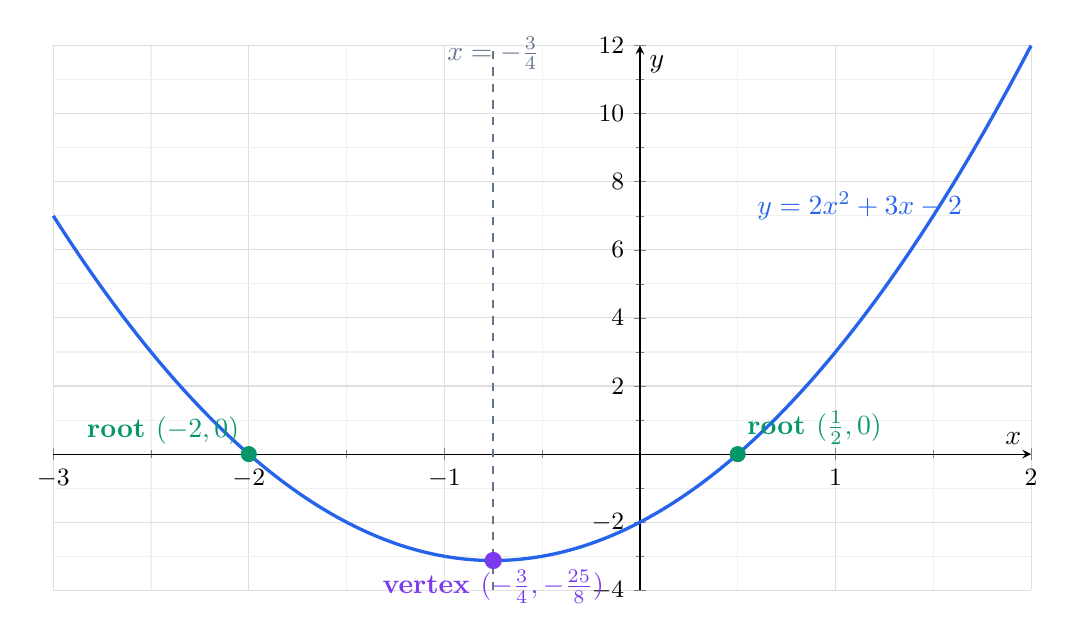
\begin{tikzpicture}
\begin{axis}[
  width=14cm,
  height=8.5cm,
  axis lines=middle,
  xlabel={$x$},
  ylabel={$y$},
  xmin=-3,
  xmax=2,
  ymin=-4,
  ymax=12,
  xtick={-3,-2,-1,0,1,2},
  ytick={-4,-2,0,2,4,6,8,10,12},
  grid=both,
  minor tick num=1,
  major grid style={draw=gray!25},
  minor grid style={draw=gray!12},
  tick label style={font=\small},
  label style={font=\bfseries},
  samples=240,
  clip=false,
]
\addplot[curveblue, very thick, domain=-3:2] {2*x^2 + 3*x - 2};
\addplot[axisgray, dashed, thick] coordinates {(-0.75,-4) (-0.75,12)};
\addplot[rootgreen, only marks, mark=*, mark size=2.7pt] coordinates {(-2,0) (0.5,0)};
\addplot[vertexviolet, only marks, mark=*, mark size=2.9pt] coordinates {(-0.75,-3.125)};
\node[anchor=south east, text=rootgreen, font=\bfseries] at (axis cs:-2,0) {root $(-2,0)$};
\node[anchor=south west, text=rootgreen, font=\bfseries] at (axis cs:0.5,0) {root $(\frac12,0)$};
\node[anchor=north, text=vertexviolet, font=\bfseries] at (axis cs:-0.75,-3.125) {vertex $(-\frac34,-\frac{25}{8})$};
\node[anchor=south, text=axisgray, font=\bfseries] at (axis cs:-0.75,11) {$x=-\frac34$};
\node[anchor=south west, text=curveblue, font=\bfseries] at (axis cs:0.55,6.6) {$y=2x^2+3x-2$};
\end{axis}
\end{tikzpicture}
\end{document}
